\documentclass[a4paper,10pt]{article}
\usepackage{graphicx}
\usepackage{amsmath}
\usepackage{hyperref}
\usepackage{caption}
\usepackage{subcaption}

\title{Computational Imaging: Camera Pipeline}
\author{David Padilla Orenga \\ Ignacio Pastore Benaim}
\date{\today}

\begin{document}
\maketitle
\thispagestyle{empty}
\newpage
\setcounter{page}{1}

\section{Image Information}
The image properties are:
\begin{itemize}
    \item Resolution: 4022 x 6024 pixels
    \item Bit depth: 16 bits per pixel
    \item Bayer pattern: RGGB (determined from metadata and visual verification)
\end{itemize}

\section{Linearization}
To linearize the image, we used the following equation:
\begin{equation}
I_{\text{linear}} = \operatorname{max}\left(0, \operatorname{min}\left( \frac{I_{\text{raw}} - \text{blackLevel}}{\text{saturationLevel} - \text{blackLevel}}, 1 \right) \right)
\end{equation}
where:
\begin{itemize}
    \item $I_{\text{raw}}$ is the original pixel intensity.
    \item $\text{blackLevel} = 1023$ (determined from metadata)
    \item $\text{saturationLevel} = 15600$ (maximum pixel intensity before clipping)
\end{itemize}

\section{Bayer Demosaicing}
The identified \textbf{RGGB Bayer pattern} was used for demosaicing. We implemented both \textbf{bilinear interpolation} and \textbf{nearest neighbor interpolation (NNI)}. 
NNI was optimized using \textbf{circshift-based propagation} significantly improving speed. Selected interpolation technique was bilinear, as it provided better color accuracy and reduced artifacts.

\section{White Balancing}
We implemented three white balancing methods:
\begin{itemize}
    \item \textbf{White World Assumption (WW)}: Assumes the brightest pixel should be pure white.
    \item \textbf{Gray World Assumption (GW)}: Assumes the average color should be neutral gray.
    \item \textbf{Manual White Balancing}: The user selects a reference point for white.
\end{itemize}
The best results were obtained using \textbf{manual white balancing}, as it provided the most natural color correction.

\section{Tone Reproduction: Brightness and Gamma Correction}
After white balancing and denoising, we applied brightness scaling \textbf{alpha correction} and contrast adjustment \textbf{gamma correction} The brightness was adjusted using:
\begin{equation}
\text{exposure\_alpha} = \log_2\left(\frac{\text{porcentage\_brighten}}{\text{max\_gray}}\right)
\end{equation}
where \textbf{porcentage\_brighten = 0.75} was selected based on visual tests, and \textbf{max\_gray} represents the highest grayscale intensity in the image. The final brightness correction was applied as:
\begin{equation}
I_{\text{alpha}} = I_{\text{color balanced}} \times 2^{\text{exposure\_alpha}}
\end{equation}

For gamma correction, we tested an \textbf{exhaustive set of combinations} for brightness and gamma values. The gamma correction follows the sRGB model:
After testing values \textbf{gamma = [1.7, 1.8, 1.9, 2.0, 2.2, 2.4]}, the best result was obtained with \textbf{gamma = 1.8} which enhanced contrast without overexposing highlights.

\section{Final Results and Compression}
Full camera pipeline is show in separate files for size purposes. We also tested different JPEG qualities to analyze 
compression ratios as shown in Table \ref{tab:compression_ratios}.
The results showed that quality levels above \textbf{75} provided visually lossless compression while achieving a high compression ratio.

\begin{table}[h!]
\centering
\begin{tabular}{|c|c|}
\hline
\textbf{JPEG Quality} & \textbf{Compression Ratio (PNG to JPEG)} \\
\hline
95 & 5.58 \\
90 & 8.83 \\
85 & 11.85 \\
80 & 14.49 \\
75 & 16.99 \\
70 & 18.87 \\
65 & 20.68 \\
60 & 22.47 \\
55 & 23.89 \\
50 & 25.13 \\
45 & 26.37 \\
40 & 28.03 \\
35 & 29.54 \\
30 & 31.54 \\
25 & 33.85 \\
20 & 36.82 \\
15 & 40.24 \\
10 & 44.89 \\
5 & 50.86 \\
\hline
\end{tabular}
\caption{Compression Ratios for Different JPEG Quality Levels}
\label{tab:compression_ratios}
\end{table}

% \begin{figure}[h]
%     \centering
%     \begin{subfigure}[b]{0.3\textwidth}
%         \centering
%         \includegraphics[width=\textwidth]{../output/IMG_0596/Linearized.png}
%         \caption{Linearized Image}
%     \end{subfigure}
%     \hfill
%     \begin{subfigure}[b]{0.3\textwidth}
%         \centering
%         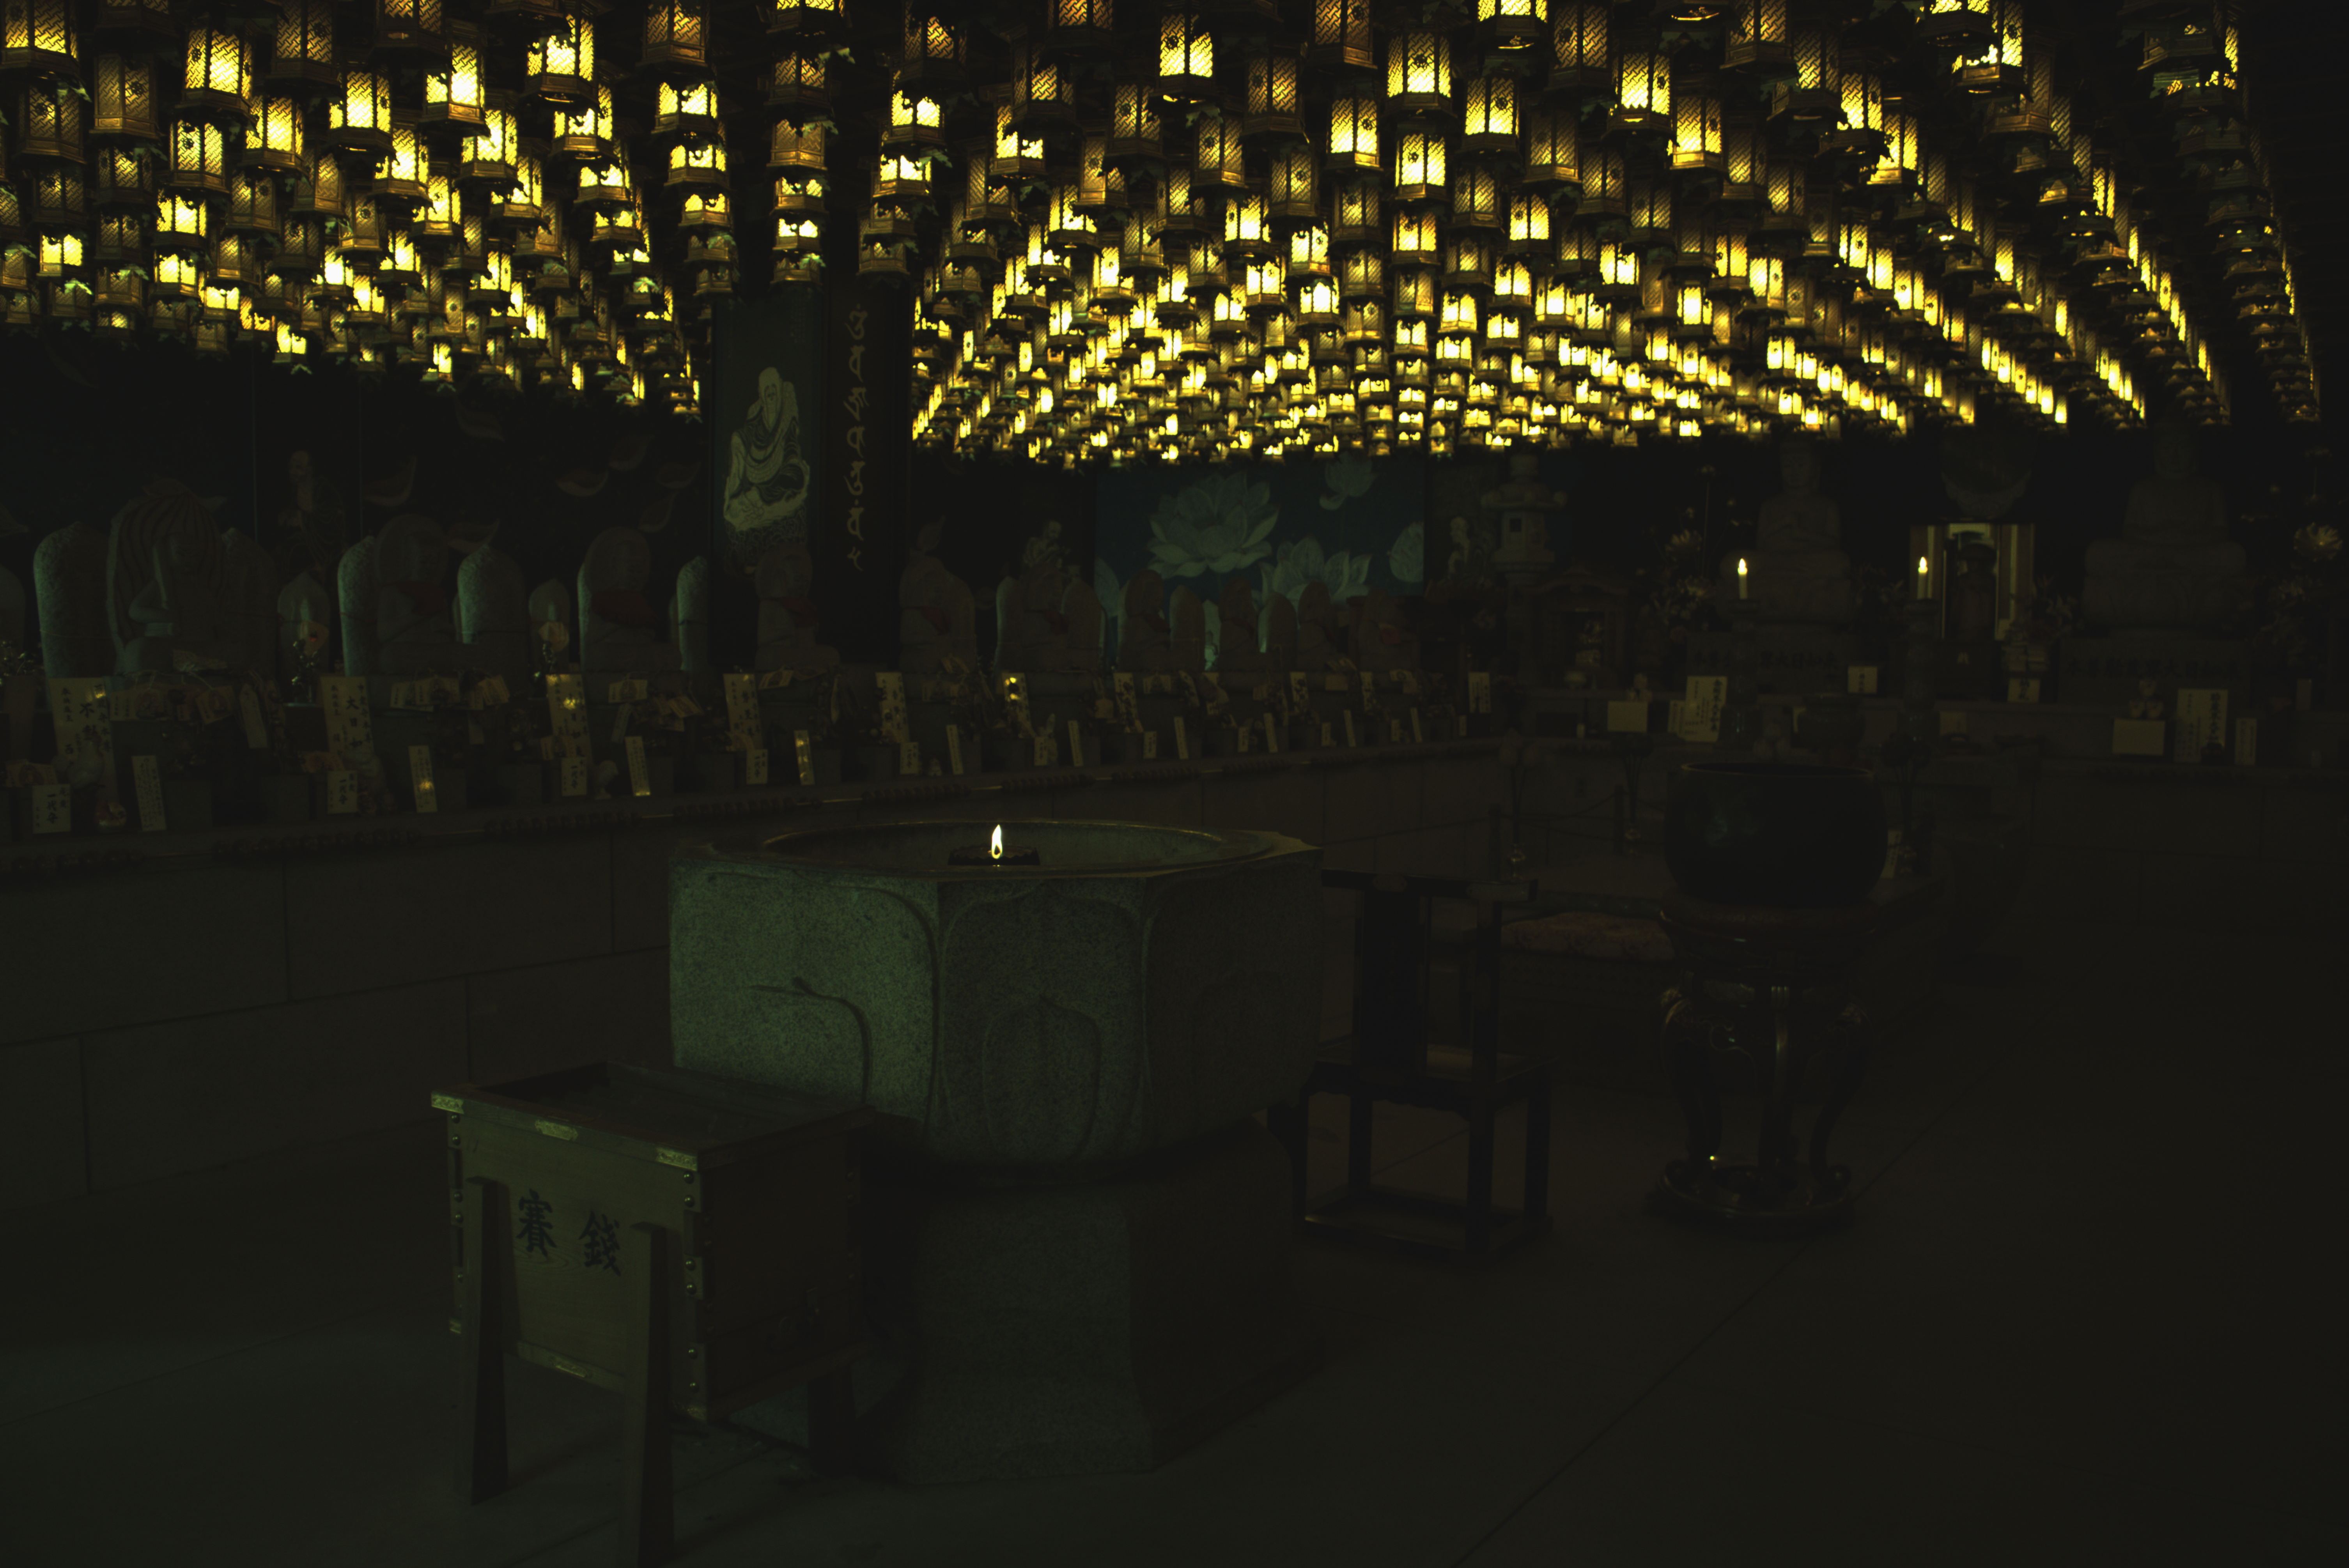
\includegraphics[width=\textwidth]{../output/IMG_0596/demosaiced_bilinear.png}
%         \caption{Demosaiced with RGGB Bayer Pattern and Bilinear Interpolation}
%     \end{subfigure}
%     \hfill
%     \begin{subfigure}[b]{0.3\textwidth}
%         \centering
%         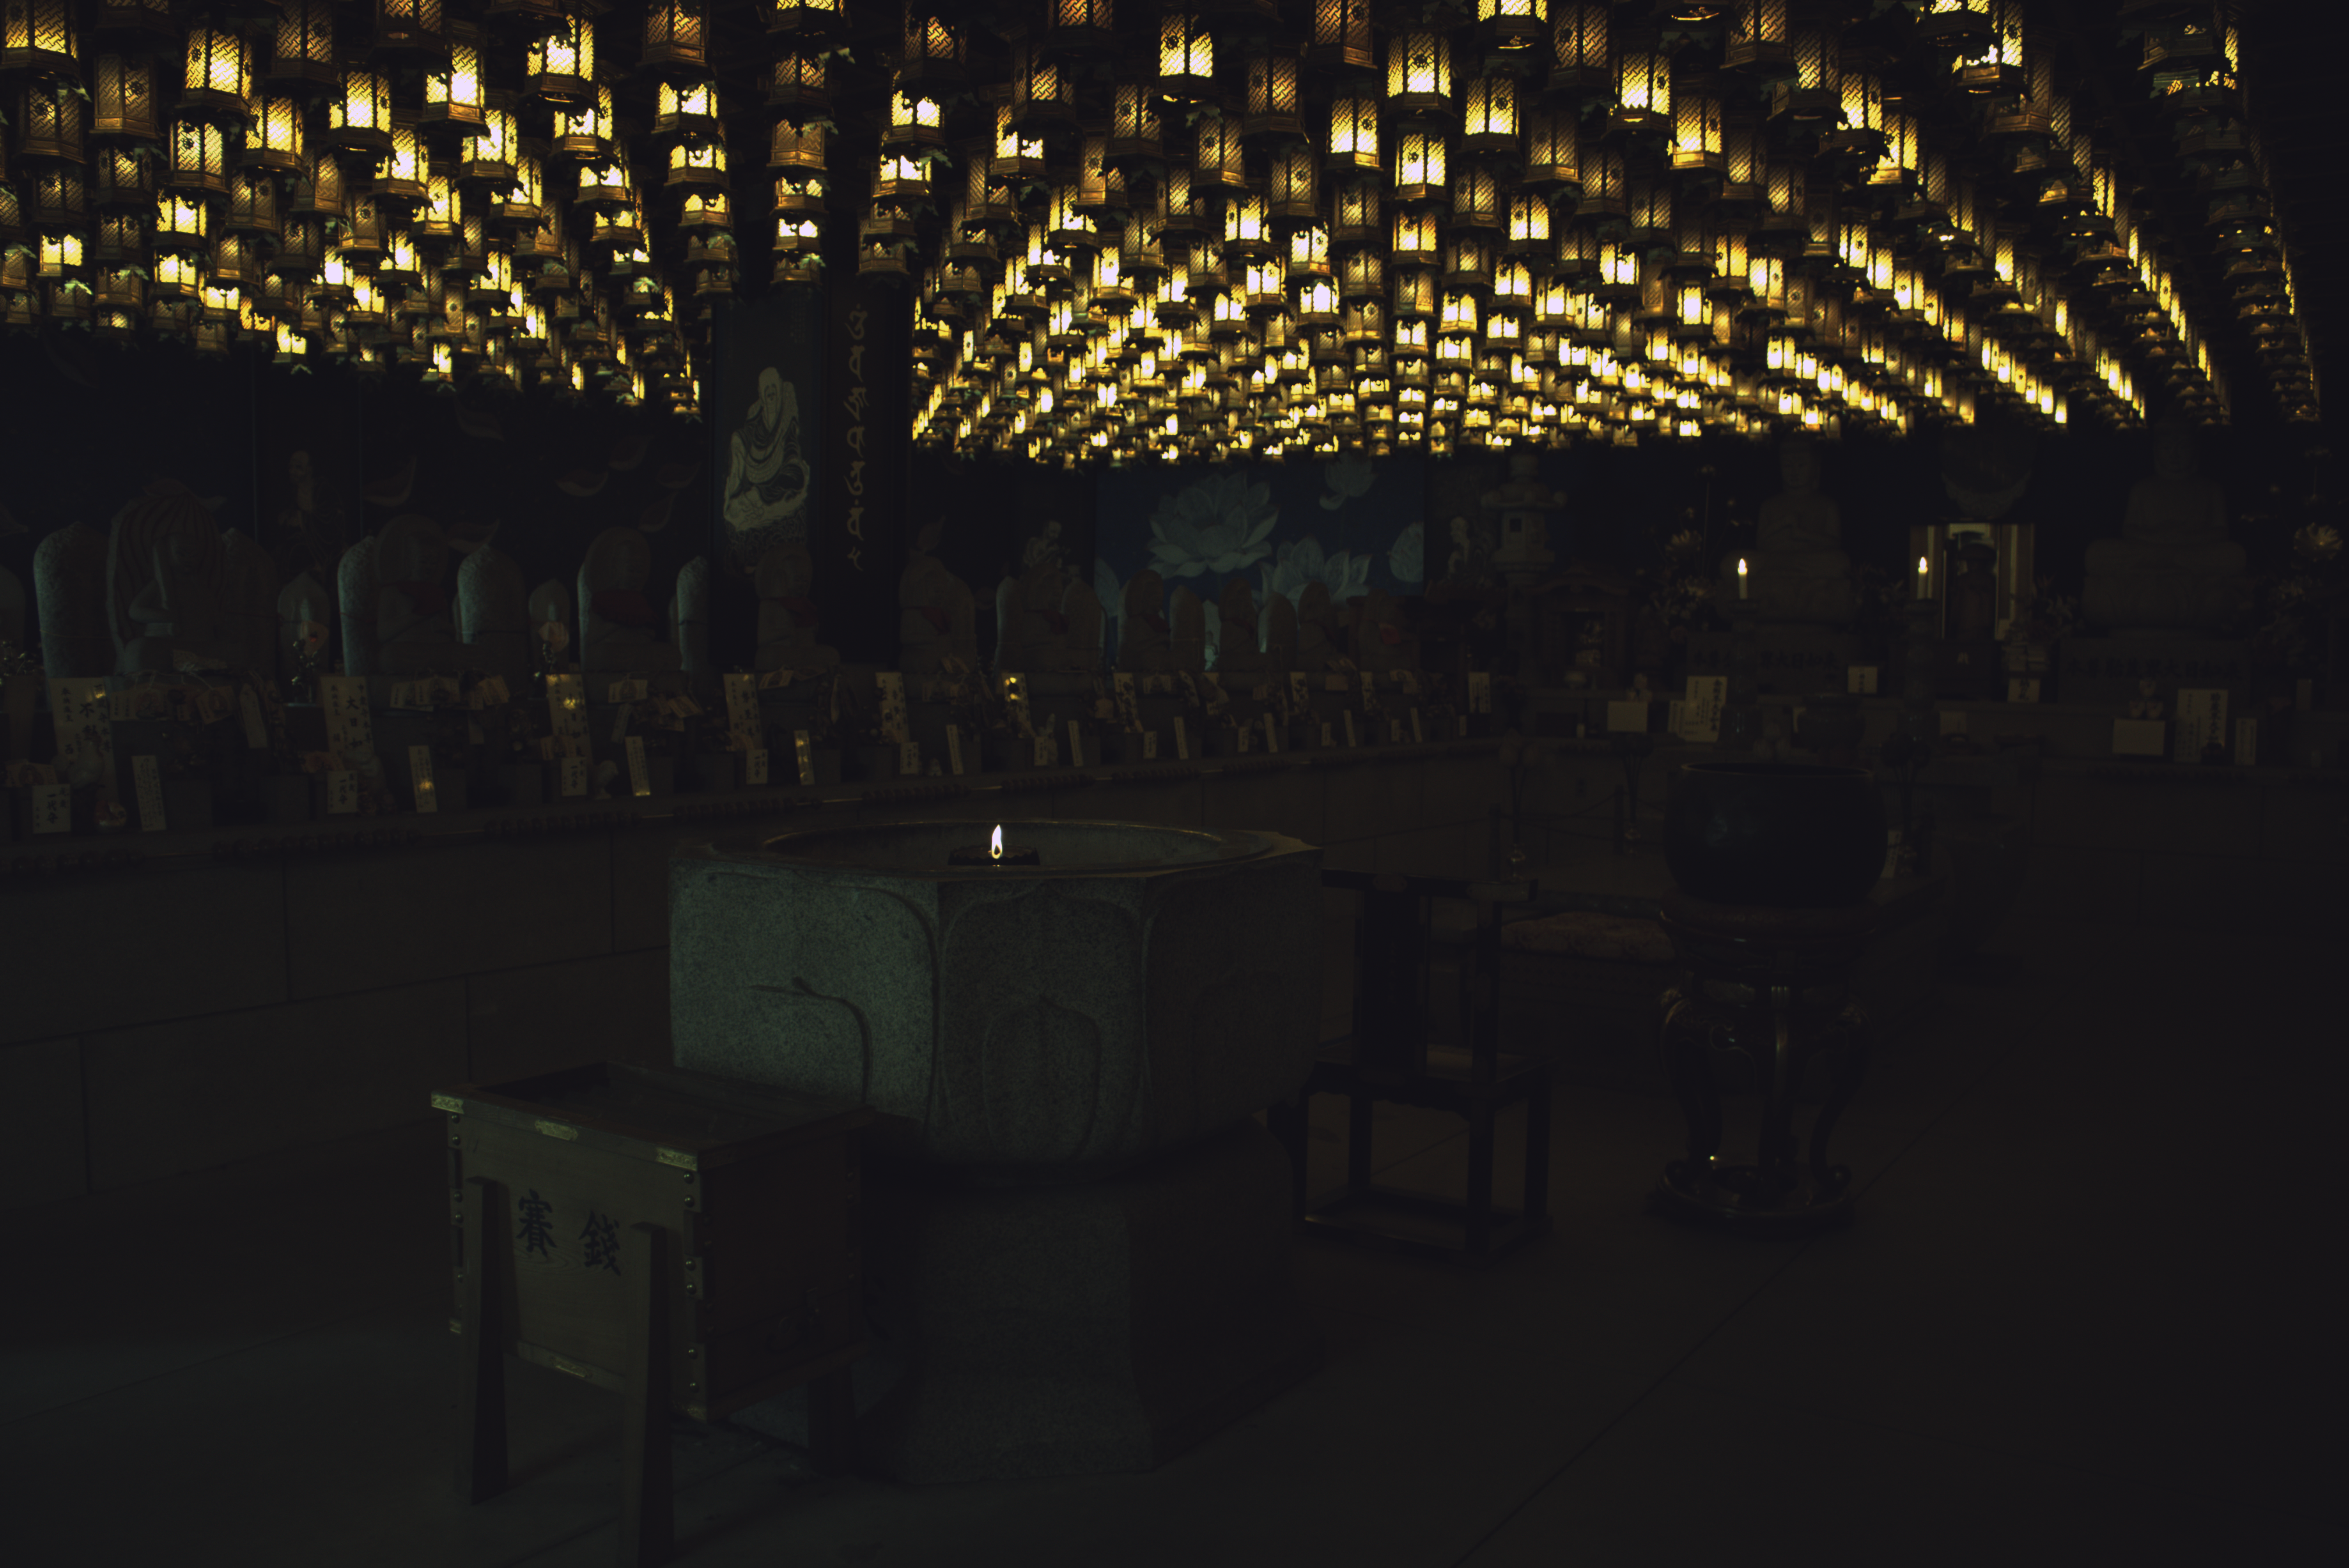
\includegraphics[width=\textwidth]{../output/IMG_0596/white_balanced_manual.png}
%         \caption{Manual White Balancing}
%     \end{subfigure}
%     \hfill
%     \begin{subfigure}[b]{0.3\textwidth}
%         \centering
%         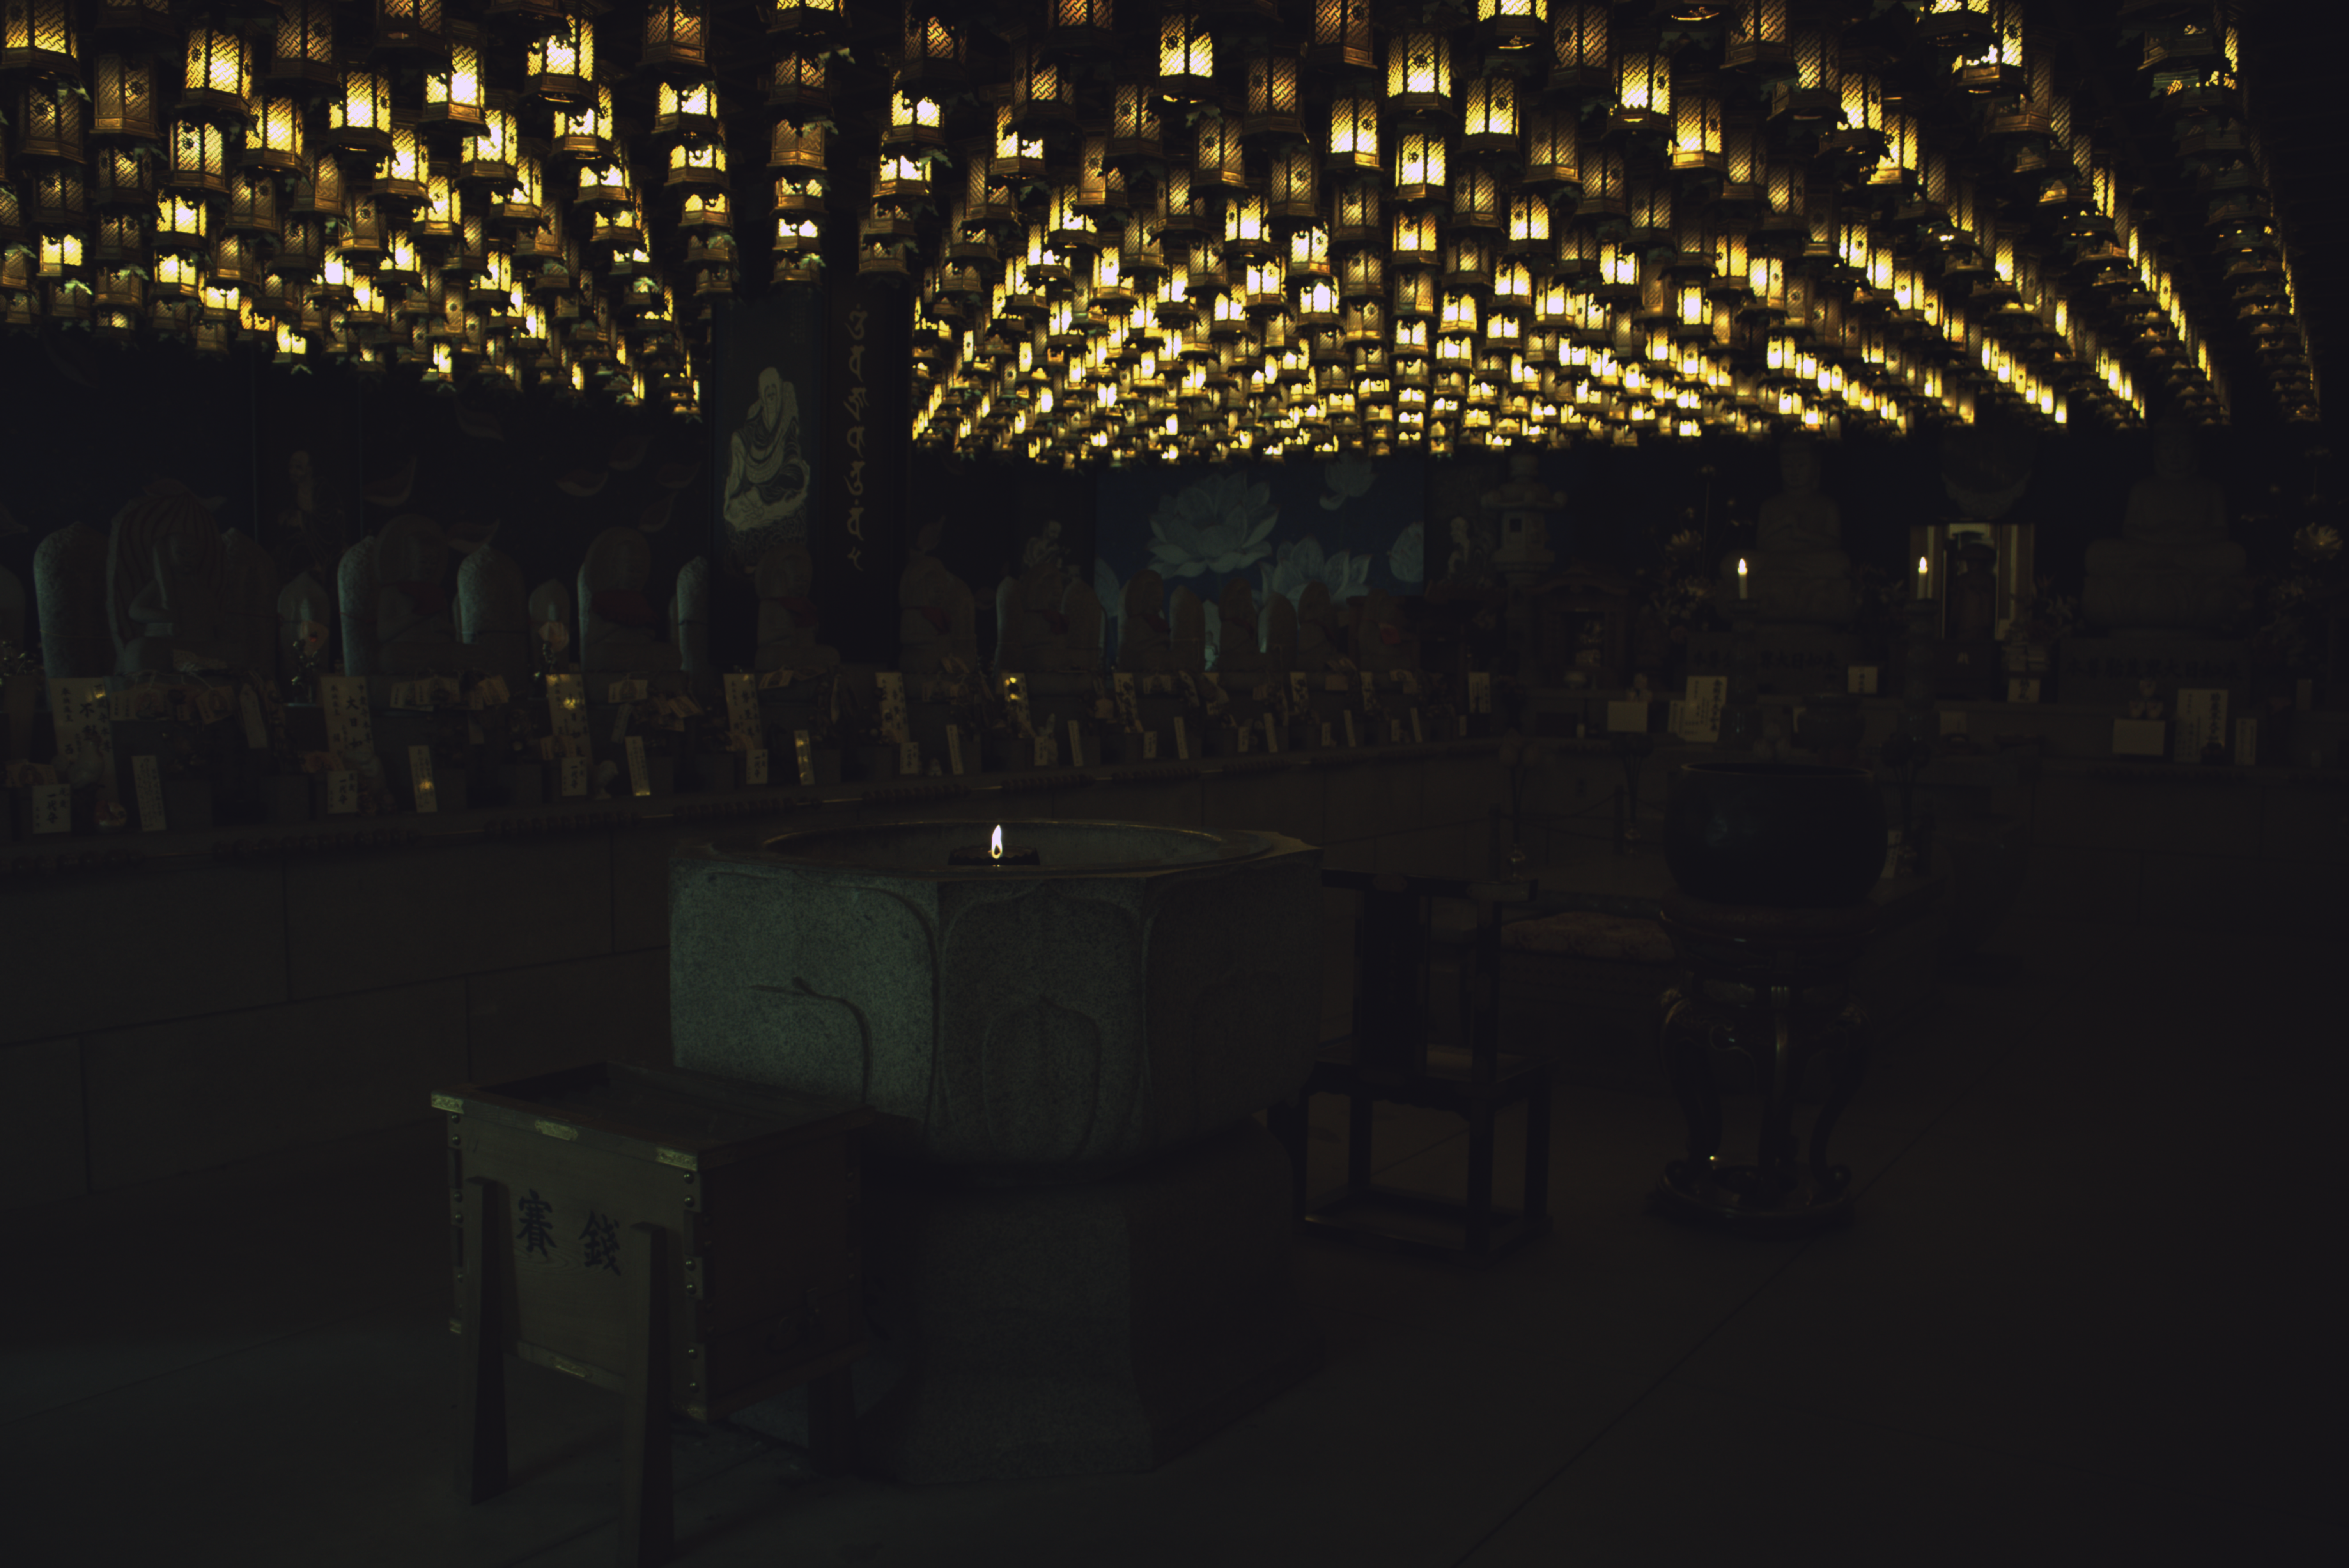
\includegraphics[width=\textwidth]{../output/IMG_0596/denoised_gaussian.png}
%         \caption{Gaussian Denoising}
%     \end{subfigure}
%     \hfill
%     \begin{subfigure}[b]{0.3\textwidth}
%         \centering
%         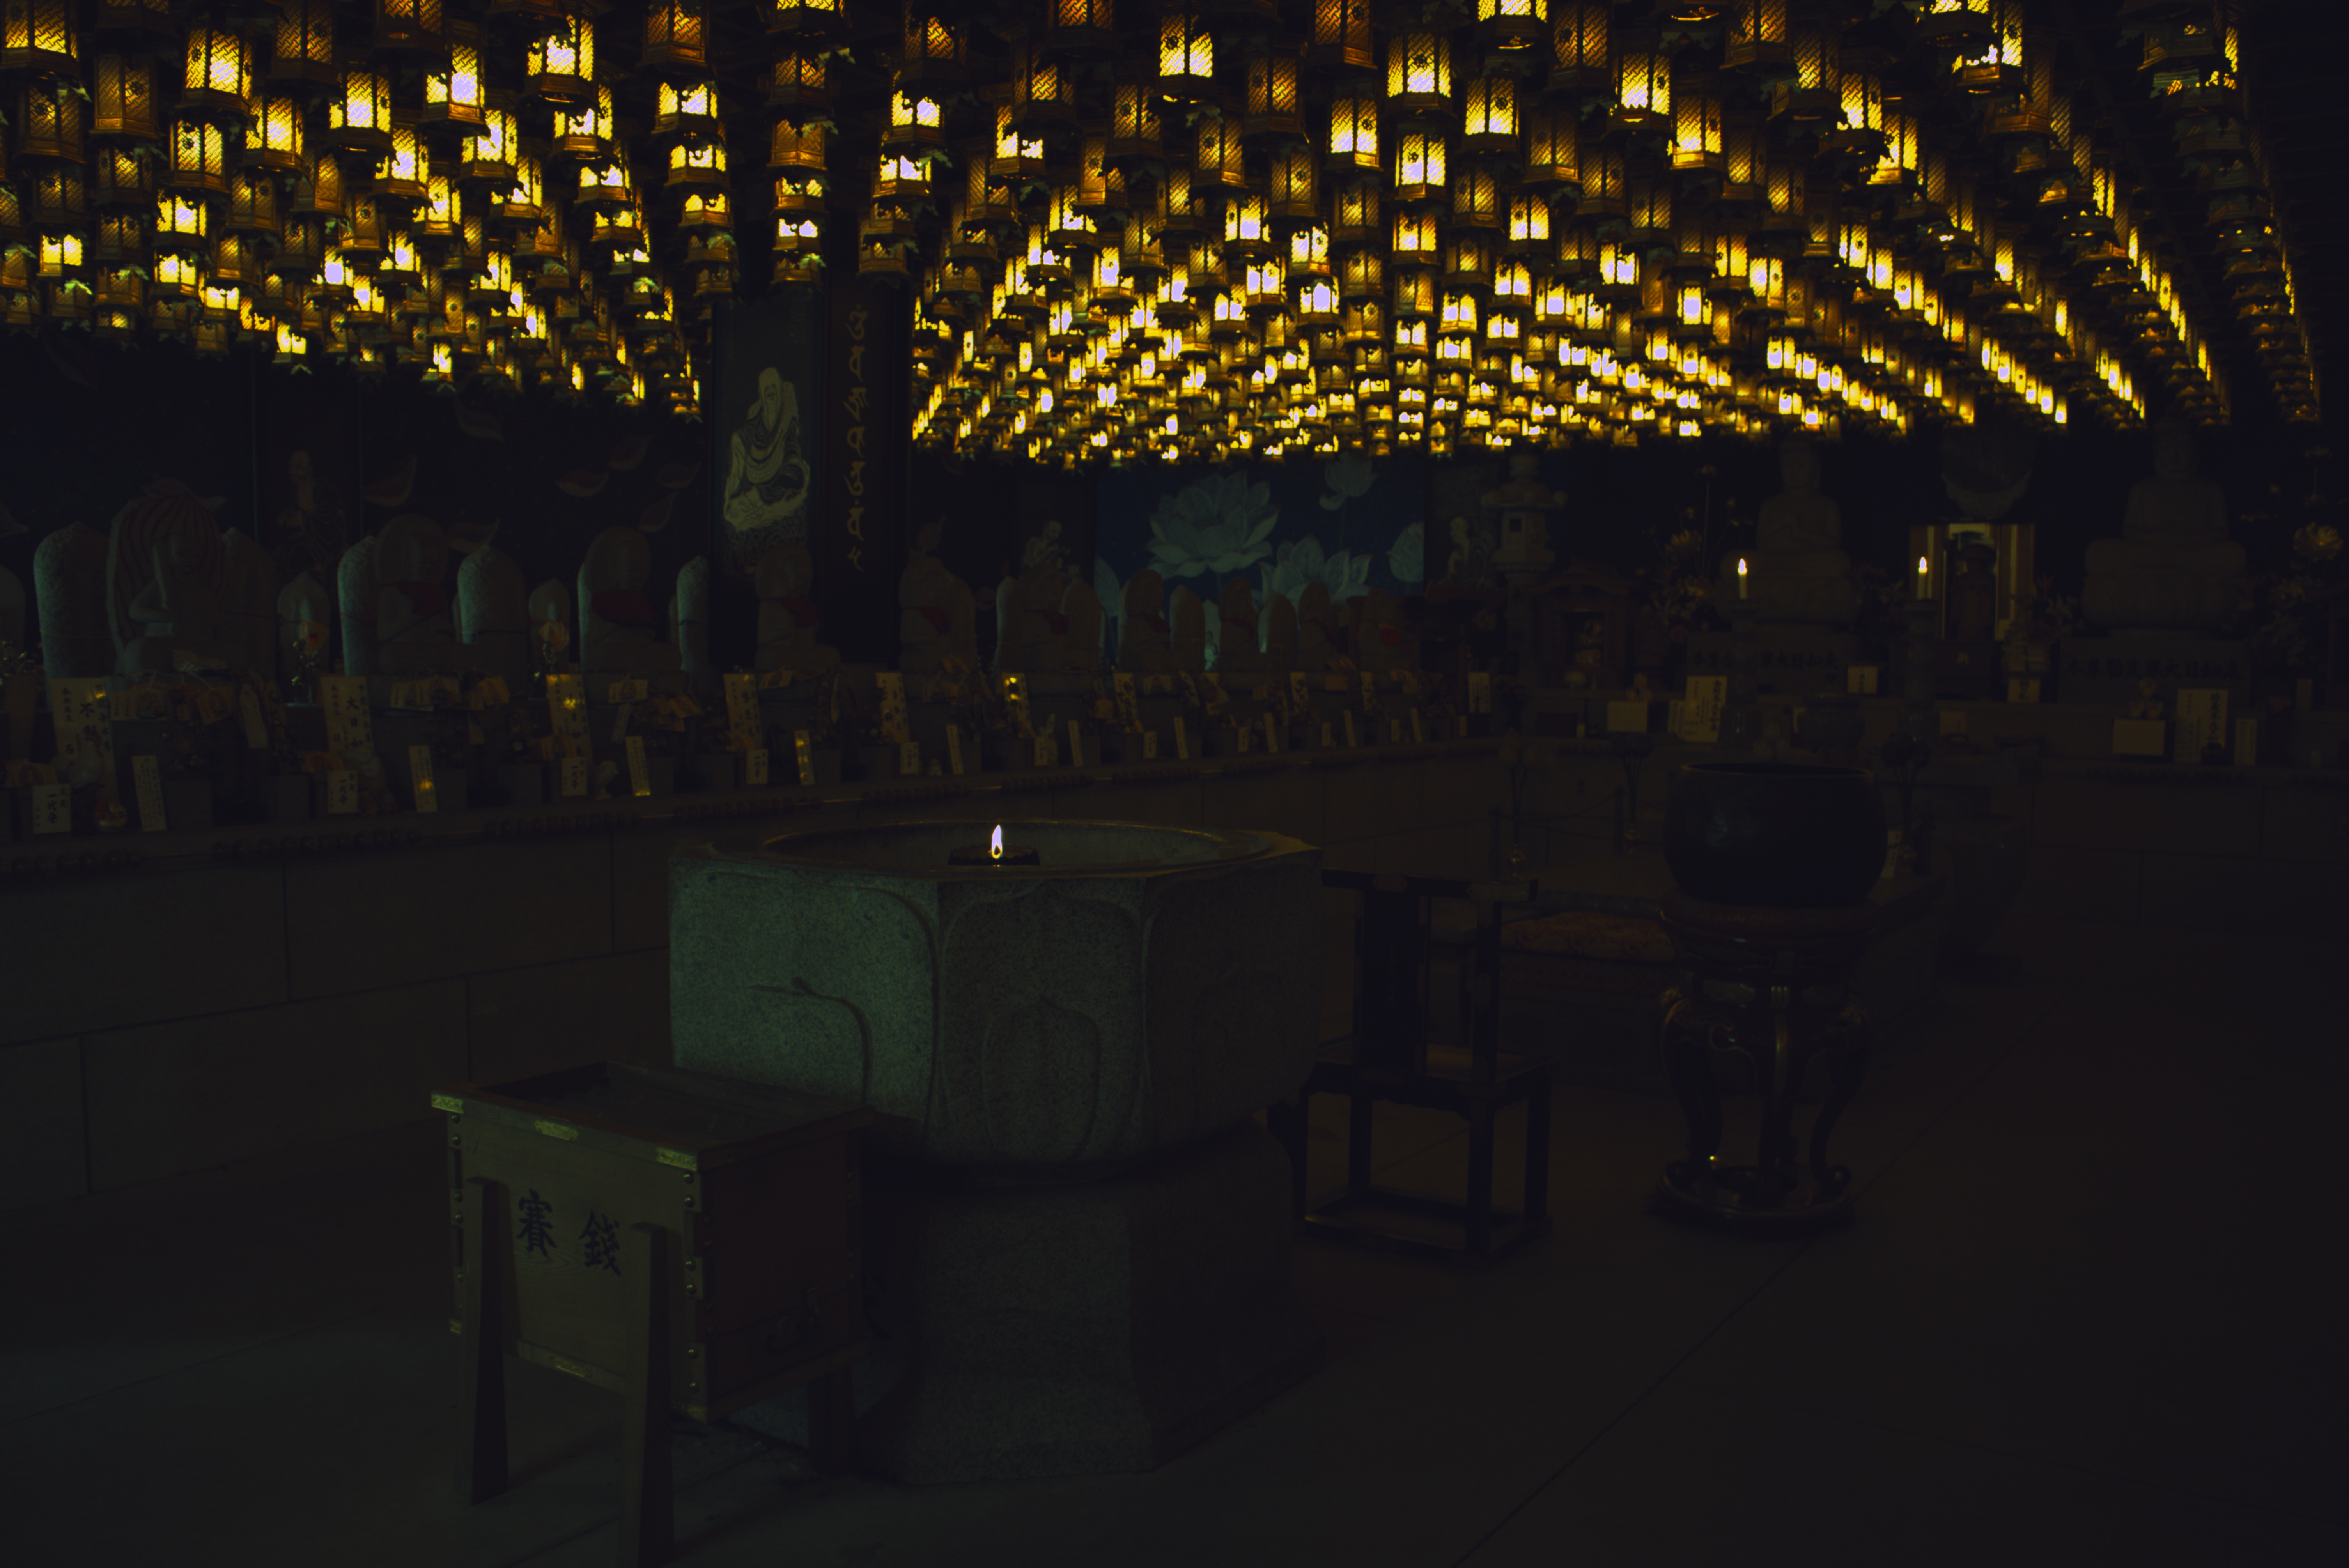
\includegraphics[width=\textwidth]{../output/IMG_0596/color_balanced_saturation_1.5.png}
%         \caption{Color Balanced with Saturation 1.5}
%     \end{subfigure}
%     \hfill
%     \begin{subfigure}[b]{0.3\textwidth}
%         \centering
%         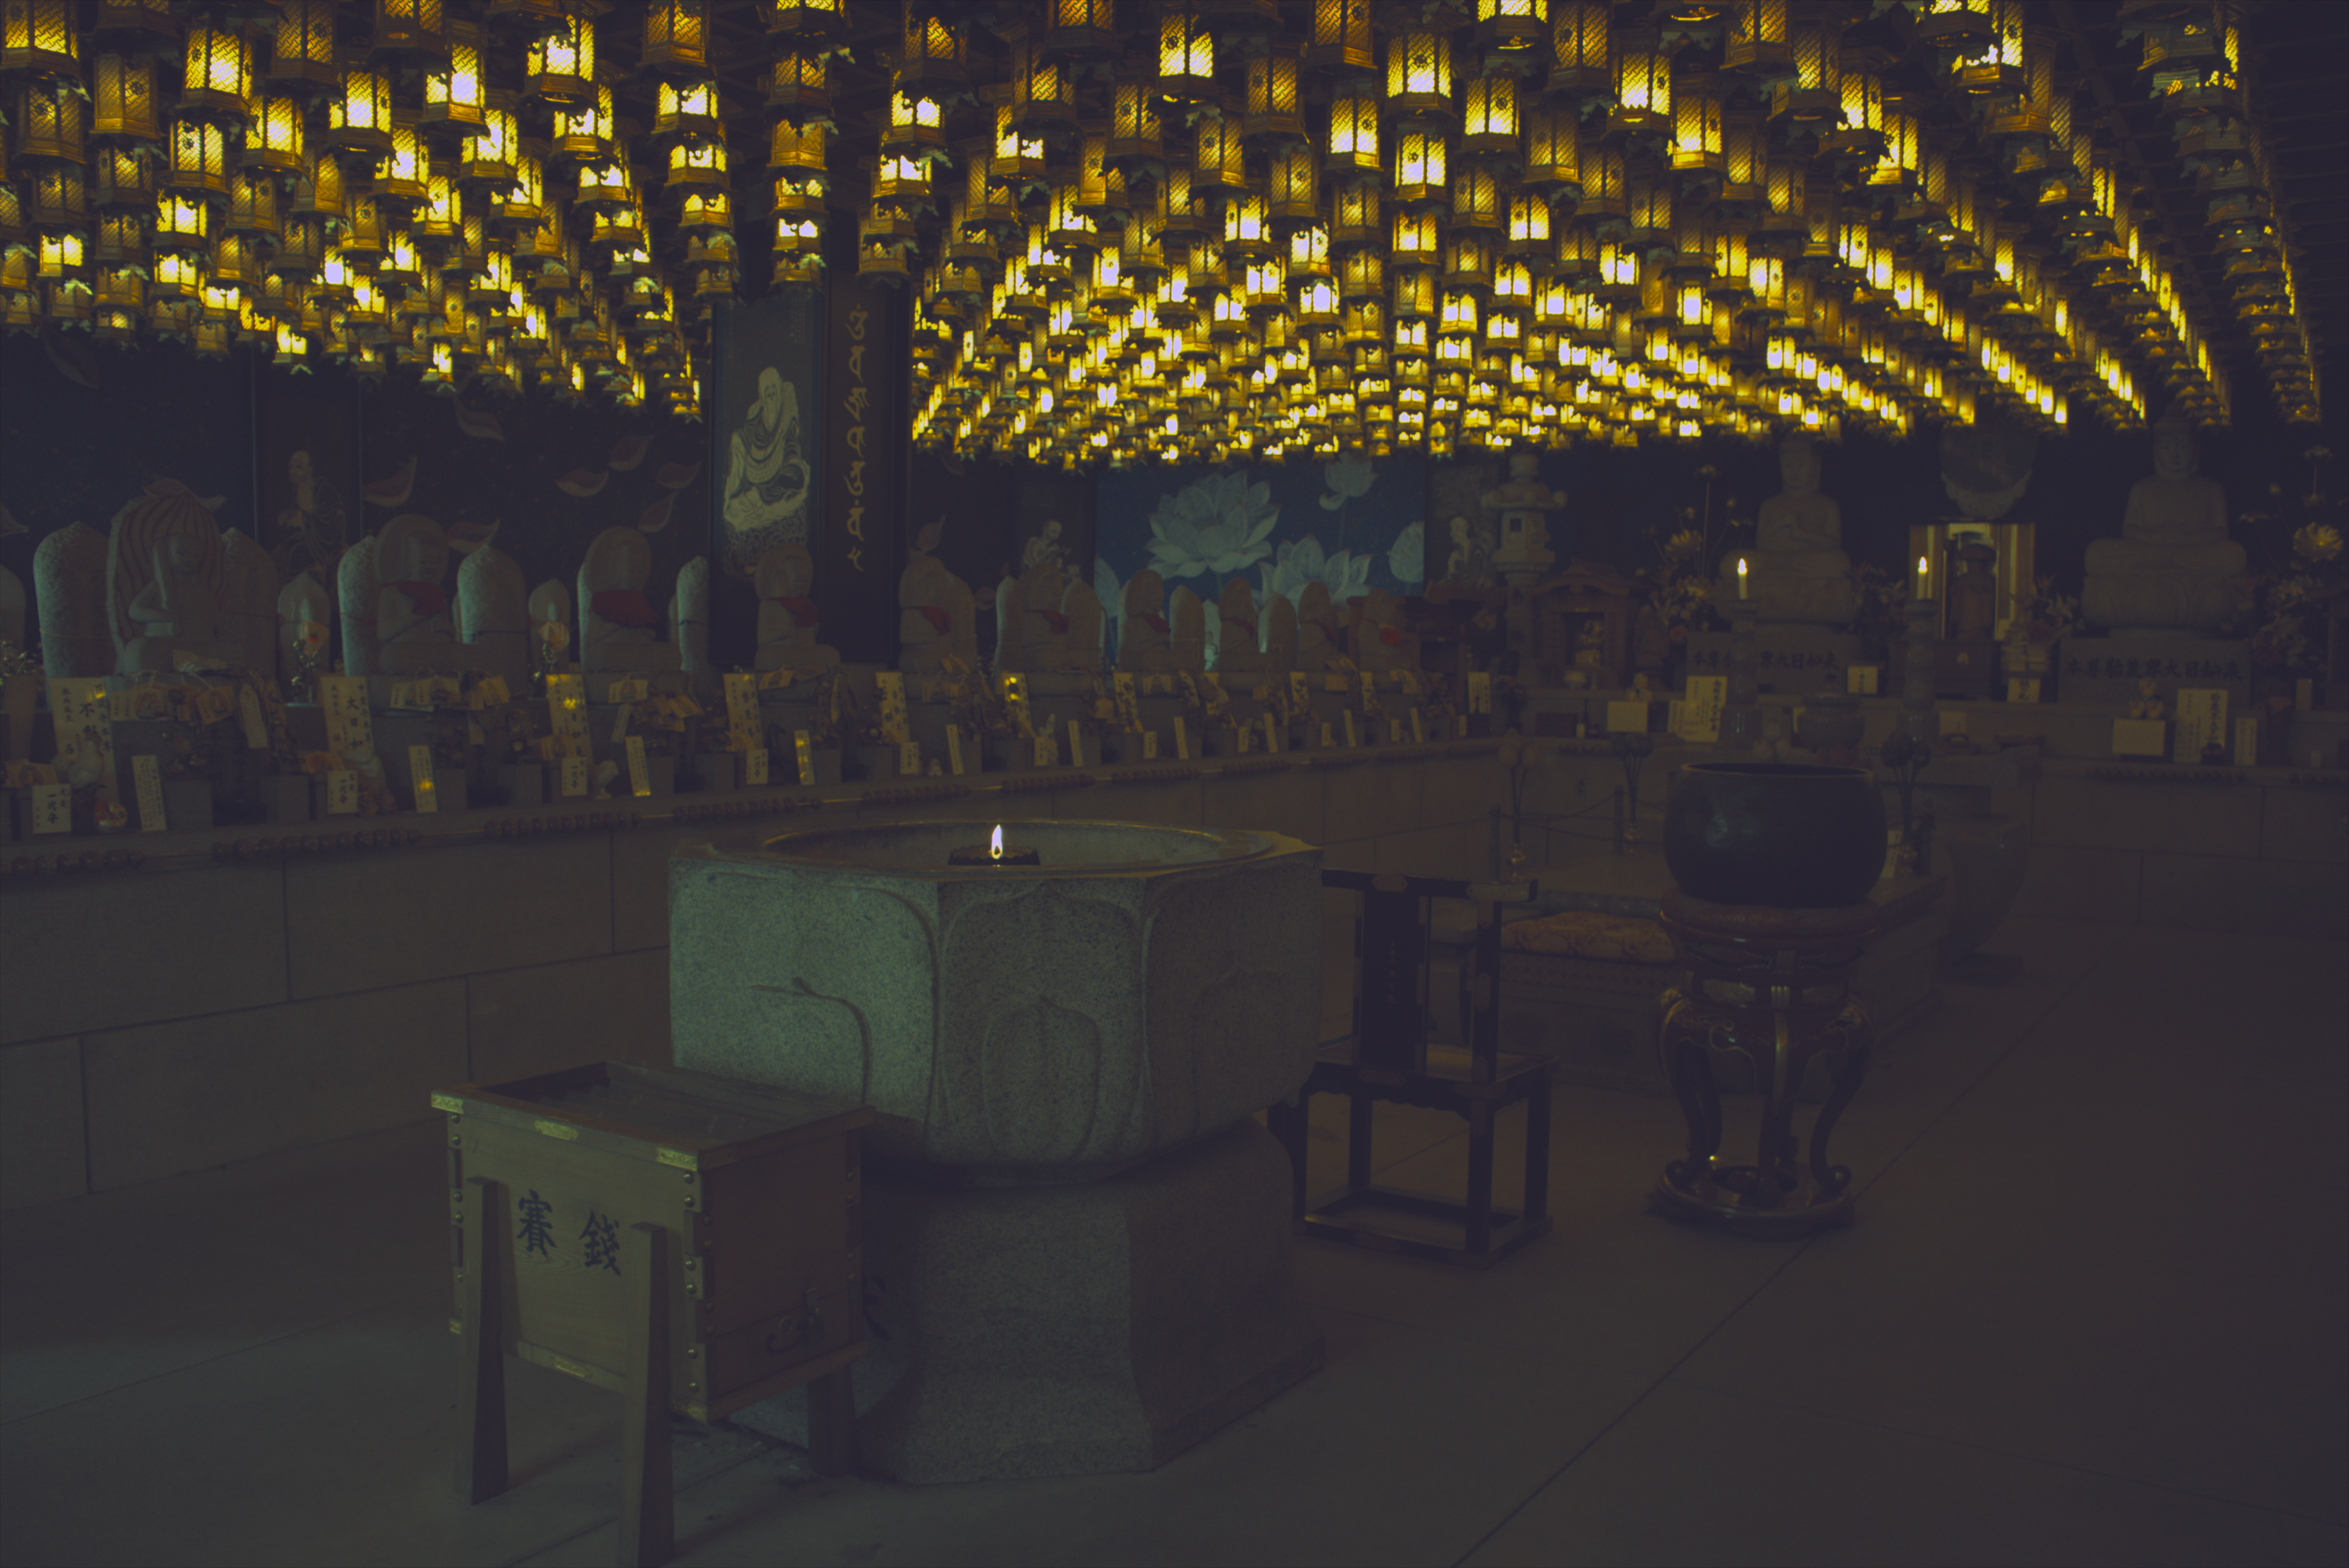
\includegraphics[width=\textwidth]{../output/IMG_0596/alpha_.75gamma_1.8.png}
%         \caption{Alpha 0.75 and Gamma 1.8 Correction}
%     \end{subfigure}
%     \hfill
%     \begin{subfigure}[b]{0.3\textwidth}
%         \centering
%         \includegraphics[width=\textwidth]{../output/IMG_0596/compressed_75.jpg}
%         \caption{Compressed to JPEG Quality 75}
%     \end{subfigure}
%     \caption{Full Camera Pipeline}
%     \label{fig:full_pipeline}
% \end{figure}

\section{Conclusion}
This pipeline successfully processed RAW images into high-quality RGB images. 
The combination of \textbf{manual white balancing, alpha correction (0.75), and gamma (1.8)} 
resulted in the best visual output. The optimized nearest-neighbor interpolation significantly 
improved performance, making the pipeline efficient for large-scale image processing.

% \begin{figure}[h]
%     \centering
%     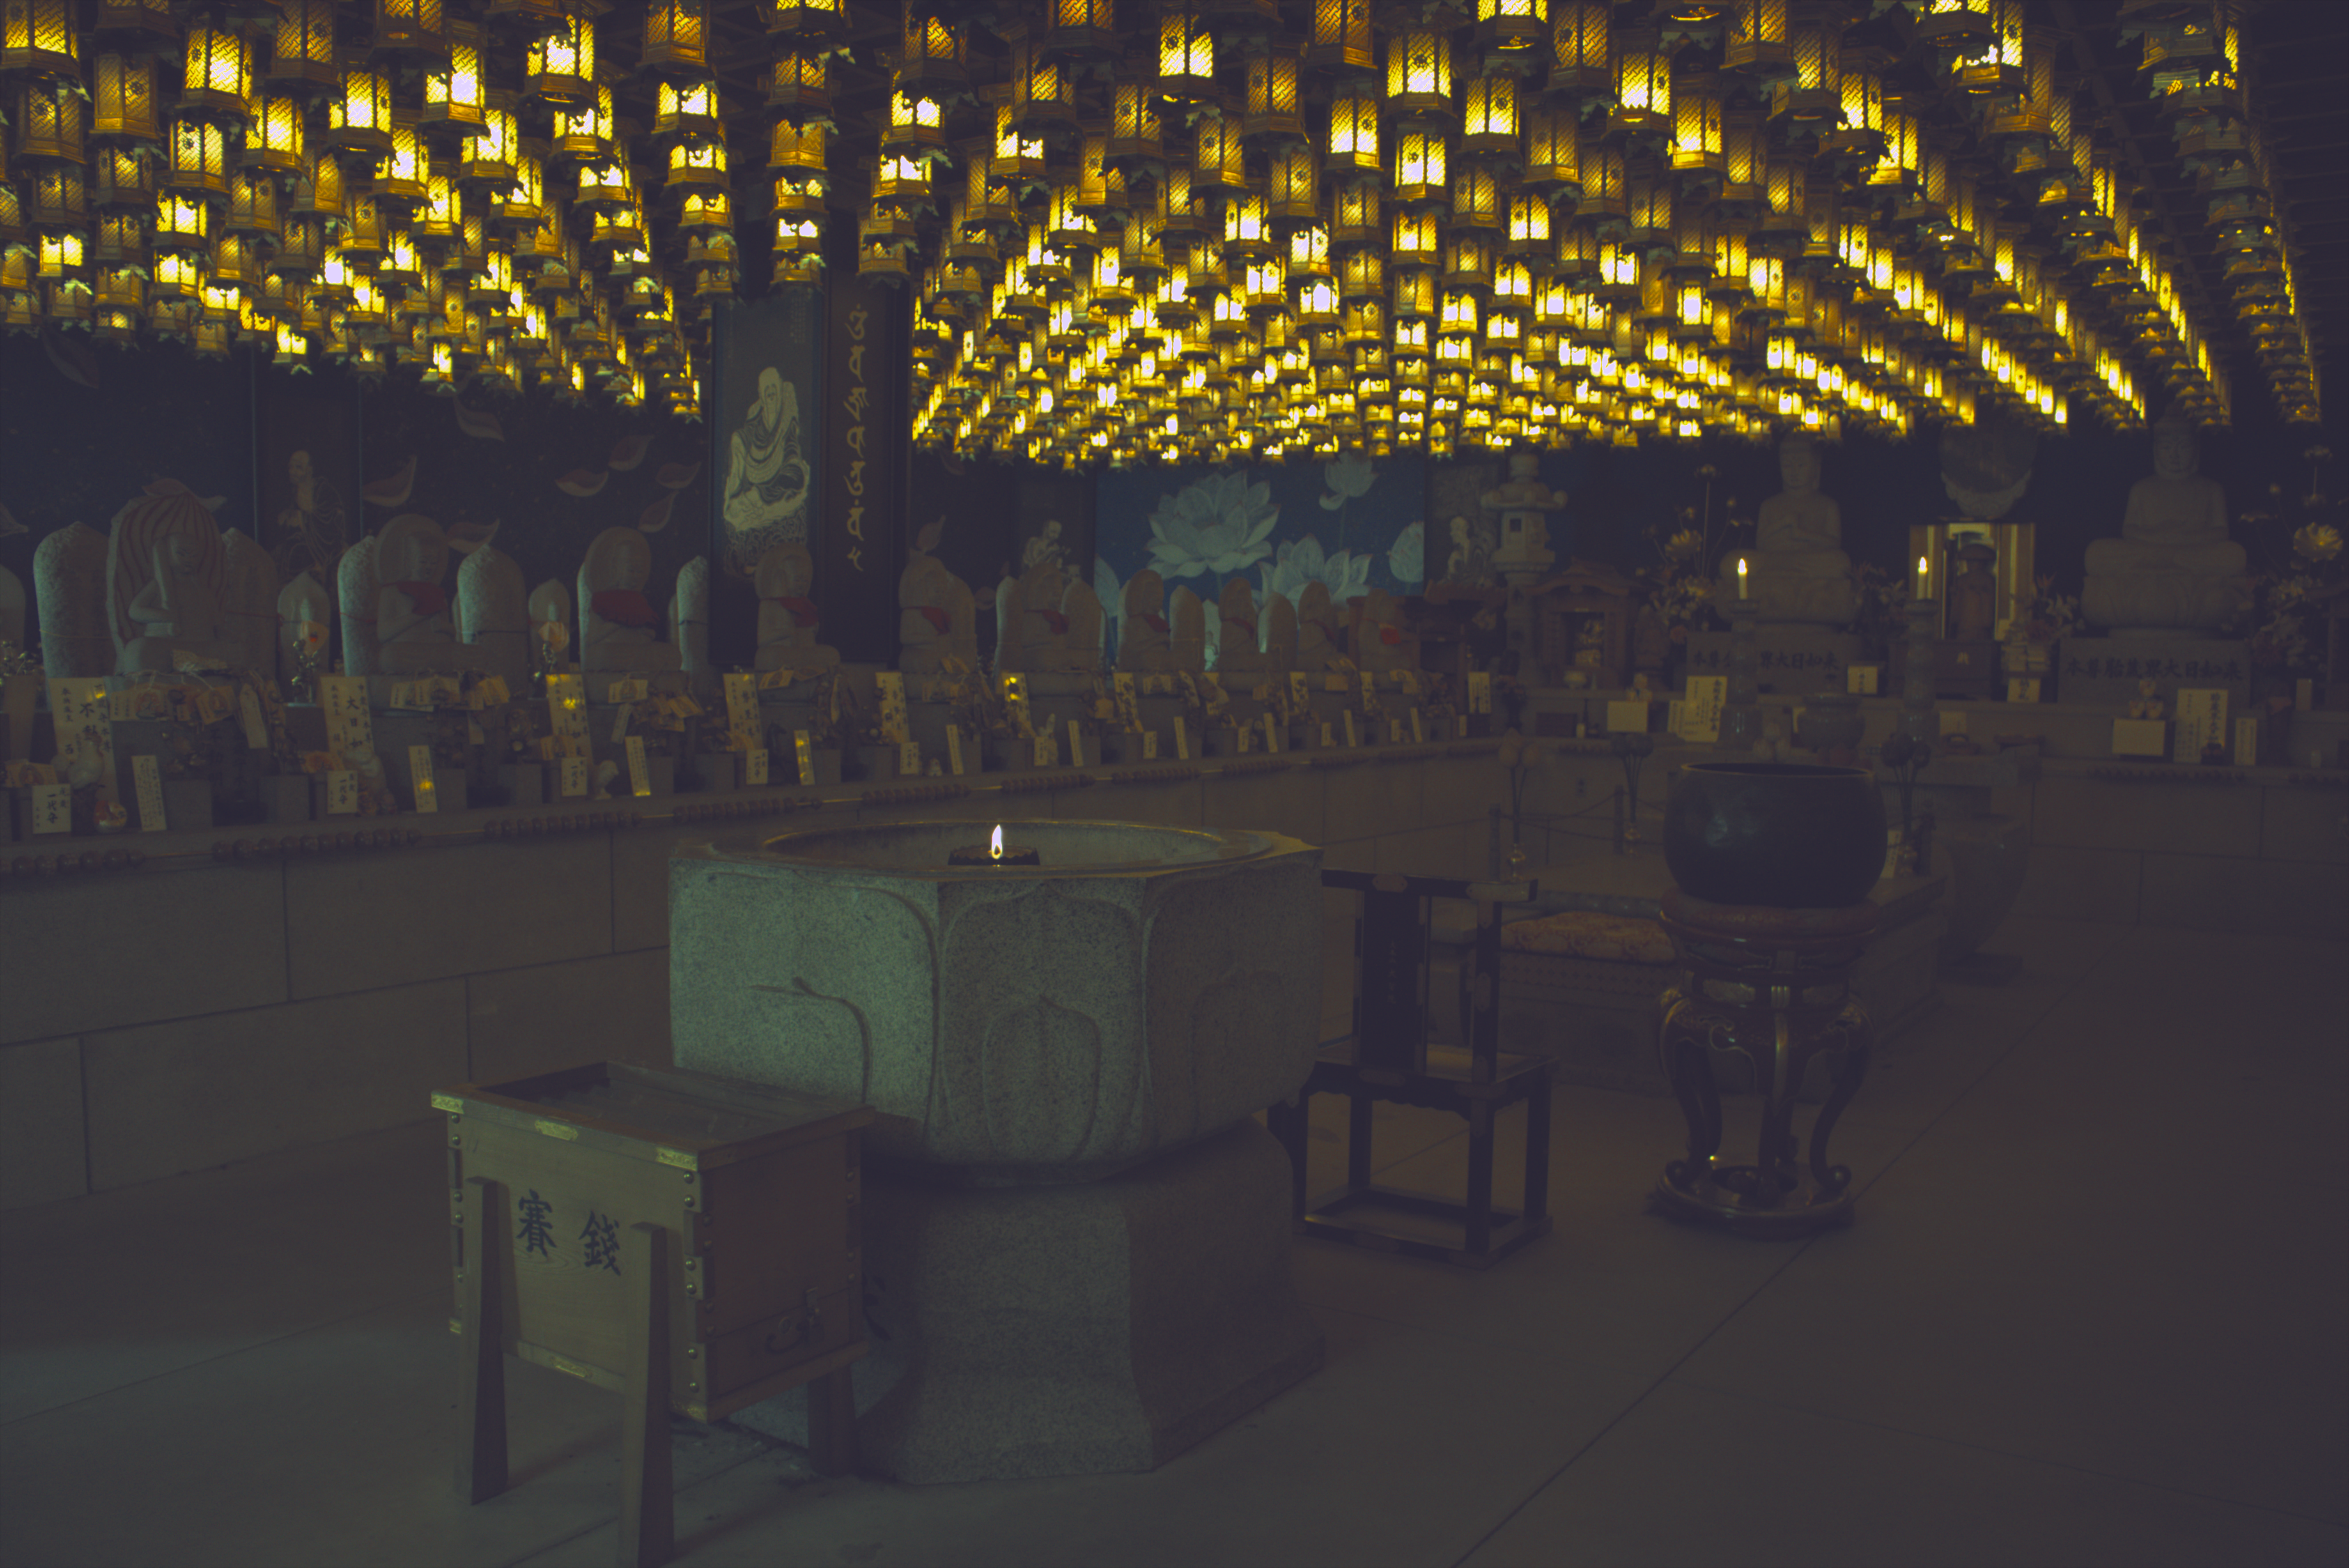
\includegraphics[width=\textwidth]{../output/IMG_0596/final_loseless.png}
%     \caption{Final Loseless Processed Image}
%     \label{fig:final_image}
% \end{figure}

\end{document}
